\documentclass{article}
\DeclareMathSizes{10}{10}{7}{7}
\usepackage{amsmath}
\usepackage{ amssymb }
\usepackage{tikz, graphicx}
\usepackage{geometry}
\usepackage[makeroom]{cancel}
\usepackage[export]{adjustbox}
\usepackage{upgreek}
\DeclareMathOperator{\sech}{sech}
\usepackage{subcaption}
\usepackage{hyperref}
\usepackage{caption}
\hypersetup{
    colorlinks=true,
    linkcolor=blue,
    filecolor=magenta,      
    urlcolor=blue,
    }
\usepackage{float}
\restylefloat{table}

\geometry{legalpaper, margin=0.7in}

\title{Surfing the waves with the mKdV equation}
\author{Liam Watson}
\begin{document}
\maketitle

\section{Introduction}
We are tasked with investigating the behavior of the so called modified KdV equation which arises in plasma's and solid-state physics.
\begin{align}
&u_t + u_{xxx} + u^2u_x = 0 \\
&u(L,t) = u(-L,t) \\
&u_x(L,t) = u_x(-L,t) \\
&u_{xx}(L,t) = u_{xx}(-L,t) \\
&u(x,0) = A \theta(\frac{1}{2}- |x|) 
\end{align}
with $\theta$ being Heavyside’s step function
\begin{align*}
\theta(x) &=
\begin{cases}
 1 & \text{if } x > 0 \\
 0 & \text{if } x \leq 0 \\
\end{cases}
\\
\theta(x) &=
\begin{cases}
 1 & \text{if } -\frac{1}{2} < x < \frac{1}{2} \\
 0 & \text{if } -\frac{1}{2} \leq x \geq \frac{1}{2}\\
\end{cases}
\end{align*}
The goals of this report are as follows:
\begin{enumerate}
\item Employ a numerical method for the equations solution 
\item Use influence functions to describe an analytical solution to the linearized equation
\item Investigate the asymptotic behavior of the KdV equation 
\item Compare the numerical and analytical results
\end{enumerate}
\section{Numerical solution}
For the numerical method we choose the sudospectral method as it exhibits better stability and performance properties. \\
Using the FD method is also a valid method and I will briefly include a derivation but not an implementation. \\
\subsection{Finite differences scheme}
\begin{align*}
&\frac{u_{j,k+1}-u{j,k-1}}{2\tau} + u^2_{j,k}\left(\frac{u_{j-1,k}-2u_{j,k}+u_{j+1,k}}{h^2} \right) + \frac{u_{j-2,k} + 2u_{j-1,k} - 2u_{j+1,k} -u_{j-2,k}}{2h^3} = 0 \\
&u_{j,k+1} = \frac{-u^2_{j,k}*2\tau}{h^2}\left(u_{j-1,k}-2u_{j,k}+u_{j+1,k} \right) - \frac{\tau}{2h^3}\left(u_{j-2,k} + 2u_{j-1,k} - 2u_{j+1,k} -u_{j-2,k} \right) + u(j,k-1)
\end{align*}
This scheme provided very poor stability and the computation time was too large to increase any hyper-parameters for better stability, hence, we will attempt to use the sudospectral method. 

\subsection{Sudospectral method}
We begin by expanding the time derivative in a center difference.
\begin{align*}
u_t = \frac{u_{j,k+1}-u_{j,k-1}}{2\tau}
\end{align*}
For the spacial derivatives we expand using a Fourier series as follows:
\begin{align*}
u_{xxx} = \sum_{n=\frac{-N}{2}}^{\frac{N}{2}-1}\left(\frac{2\pi i n}{L}\right)^3 \widehat{u_n}(t_k)e^{\frac{2\pi i n j}{N}}
\end{align*}
The nonlinear term is not quite as simple but we can, after a little effort find a Fourier series representation for it. Notice that:
\begin{align*}
u^2u_x = \frac{\partial}{\partial x}\left(\frac{u^3}{3}\right)
\end{align*}
We call the expression in the brackets $f(x,t)$ which we expand in a Fourier Series.
\begin{align*}
f(x,t) = \sum_{n=\frac{-N}{2}}^{\frac{N}{2}-1}\left(\frac{2\pi i n}{L}\right) \widehat{\left(\frac{u^3}{3}\right)}_n(t_k)e^{\frac{2\pi i n j}{N}}
\end{align*}
We now have expressions for all the terms in the modified KdV equation and can implement a numerical solution. 

For completeness the implementation of the sudo spectral method can be found \href{https://github.com/Liam-Watson/Analysis-of-mKdV-equation-with-Heaviside-IC/blob/main/a.m}{here}.\\
To test the method we must simulate the evolution of the Heaviside initial condition. We will use $A = 0.3$. There was significant complexity with ensuring a stable numerical solution due to the highly discontinuous IC. \\
A note on the graphics used in this paper: All heat maps show $t$ on the vertical axis and $x$ on the horizontal. The surface plots show amplitude on the $z$ axis, $t$ on the depth axis and $x$ on the horizontal axis.  
\begin{figure}[H]
\centering
\begin{subfigure}[b]{60mm}
\includegraphics[scale=0.1]{figures/smallTime.png}
\caption{Small time plot of $u(x,t)$ with A = 2, L = 30 and standard time step size. }
\label{fig:}
\end{subfigure}
\begin{subfigure}[b]{60mm}
\includegraphics[scale=0.1]{figures/bigTime.png}
\caption{Large time plot of $u(x,t)$ with A = 2, L = 30 and standard time step size.}
\label{fig:}
\end{subfigure}
\caption{In sub figures (a) and (b) we can see significant instability. The solution grows rather than dispersing and we notice highly erratic waves forming for a coarse x-mesh}
\label{fig:}
\end{figure} 
However all is not lost, if we increase the interval size, shift the solution to the positive x region by $L/2$ and ensure our $x$ and $t$ are partitioned into a fine enough mesh. We can produce the following numerical solution.
\begin{figure}[H]
\centering
\begin{subfigure}[b]{80mm}
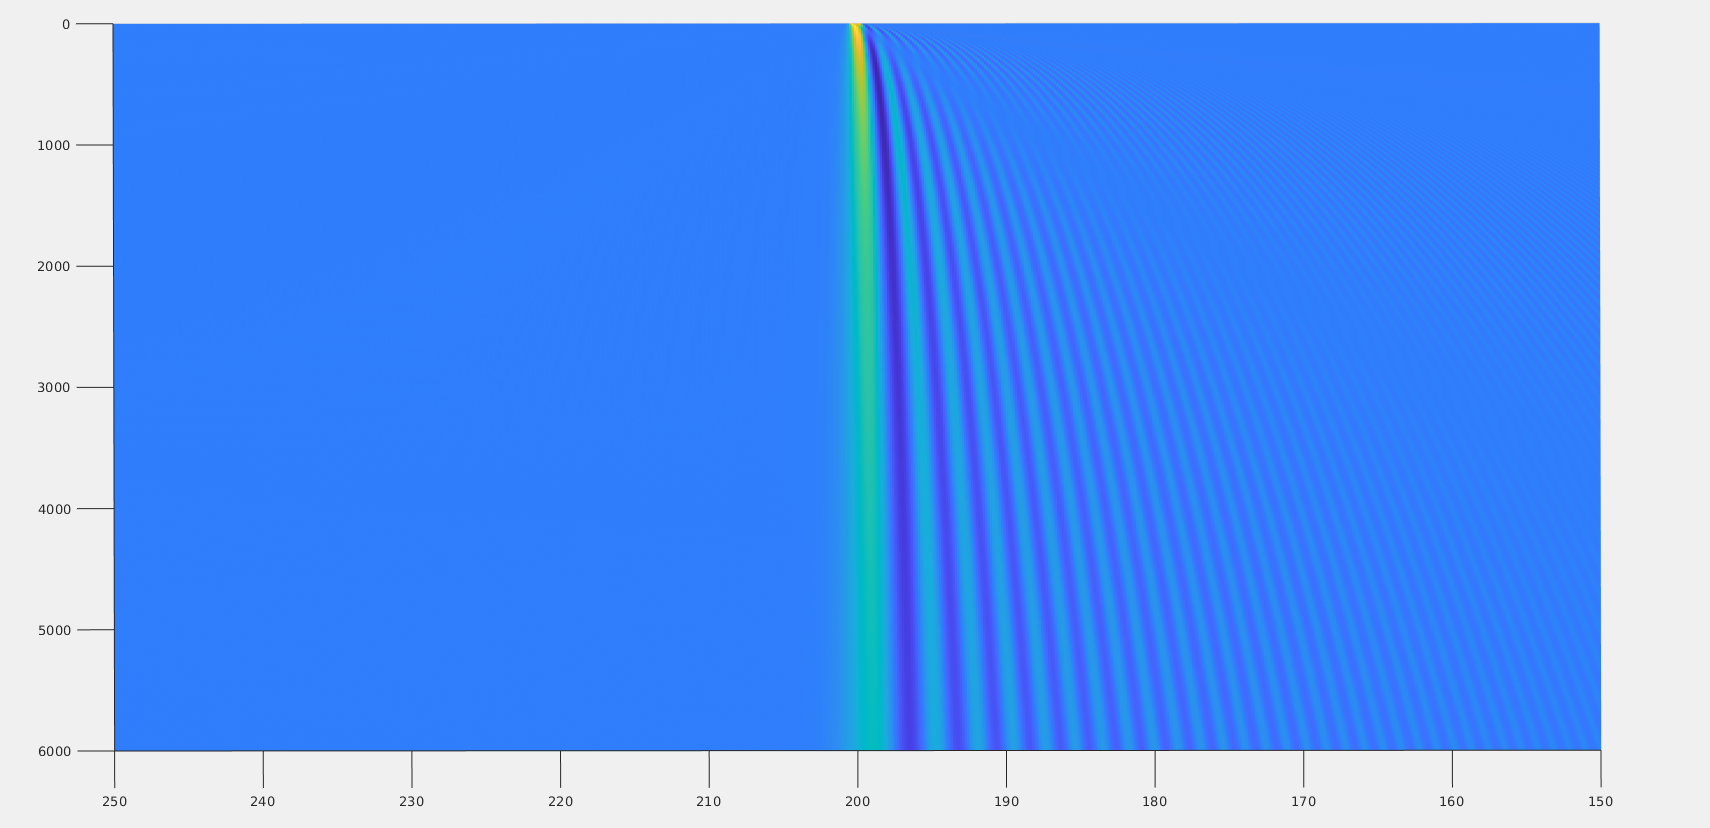
\includegraphics[scale=0.13]{figures/simL400.png}
\caption{Heat mat showing that the initial condition disperses over time. We can see the initial condition disperses as time progresses due to the blue shift in hue.}
\label{fig:}
\end{subfigure}
\begin{subfigure}[b]{80mm}
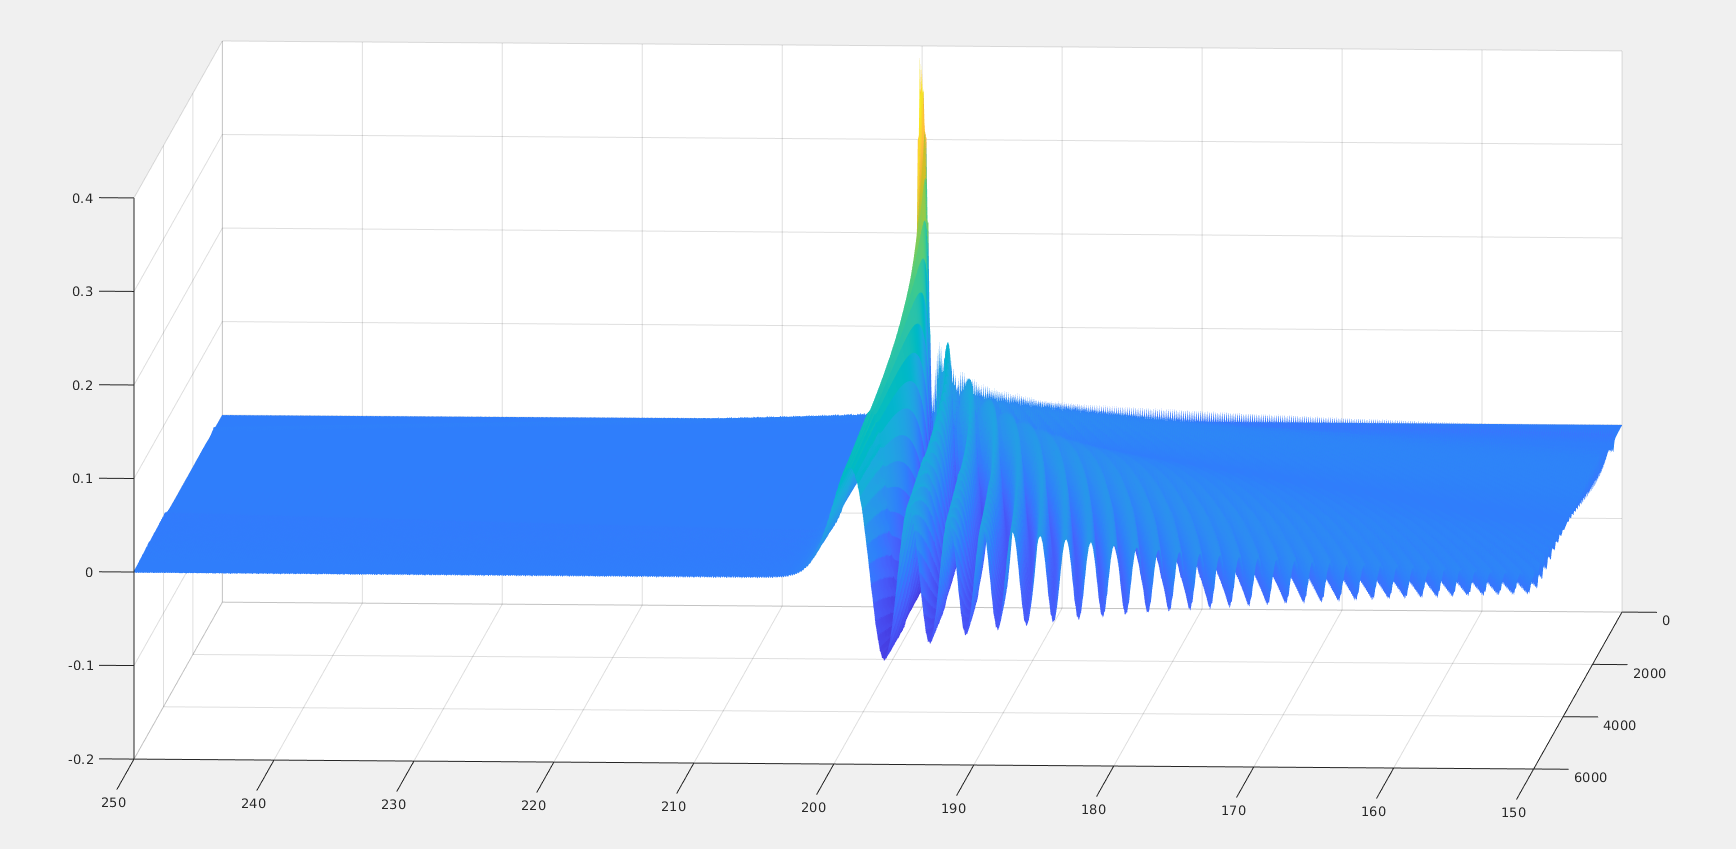
\includegraphics[scale=0.12]{figures/3DsimL400.png}
\caption{A surface plot showing that the initial condition disperses into many smaller waves over time, reducing in amplitude}
\label{fig:}
\end{subfigure}

\caption{In sub figures (a) and (b) we can see that most instability has been removed by the changes and now we can clearly see the dispersive property of the mKdV equation. }
\label{fig:}
\end{figure} 

Note that other attempts to resolve the initial conditions resistance to integration were made such as a Fourier series approximation of a square wave or $A\sech(cx^b); c,b\in \mathbb{R}_+$ however, these smooth approximations did not aid the integrability of the initial condition to a large enough degree to justify the loss in rigor.  
\section{Analytic solutions}
In this section we assume that $A$ is small $A^2\approx0.1$ and as such the non-linearity should be negligible compared to the dispersion and we can get a good approximate analytical solution by solving the linearized KdV equation with the same IC and BC's:
\begin{align*}
&u_t + u_{xxx} = 0
\end{align*}
\subsection{Influence equation}
First to find the influence function we must assume that a Fourier transform exists as follows
\begin{align*}
&u(x,t) = \int U(k,t)e^{-ikx}dk
\end{align*}
The we assume that we can differentiate under the integral to find that
\begin{align*}
&u_{xxx} = \int (-ik)^3U(k,t)e^{-ikx}dk \\
&u_t = \int U_t(k,t)e^{-ikx}dk
\end{align*}
Putting the above expressions for $u_{xxx}$ and $u_t$ back into the linearized KdV equation we find that
\begin{align*}
\int (U_t + ik^3 U) e^{-ikx}dk = 0
\end{align*}
We know the Fourier Transform of zero is zero so the integrand must be zero. The integrand is a simple linear ODE in time which we can easily solve:
\begin{align*}
U_t + ik^3U = 0 \implies U(k,t) = F(k)e^{ik^3t}
\end{align*}
Now that we know $U(k,t)$ we can put it into the expression we had for $u(x,t)$.
\begin{align*}
u(x,t) = \int F(k) e^{ik^3t}e^{-ikx}dk
\end{align*} 
Next we need to determine $F(k)$ using the IC and we find
\begin{align*}
F(k) &= \frac{1}{2\pi} \int_{\infty}^{\infty} f(x^\prime) e^{ikx^\prime}dx^\prime \\
&= \frac{A}{2\pi} \left[ \int_{-\infty}^\frac{-1}{2} 0e^{ikx^\prime}dx^\prime        \int_\frac{-1}{2}^\frac{1}{2}e^{ikx^\prime}dx^\prime \int^{\infty}_\frac{1}{2} 0e^{ikx^\prime}dx^\prime\right] \\
&= \frac{A}{2\pi}\int_{-\frac{1}{2}}^\frac{1}{2}e^{ikx^\prime}dx^\prime \\
&= \frac{A}{2\pi}\frac{2\sin(\frac{k}{2})}{k}
\end{align*}
We now need to use the Convolution theorem to determine the influence function. We notice that the integrand is close to the Airy function Fourier Transform $e^{\frac{ik^3}{3}}$. We can form an equation so satisfy both the convolution theorem and the Airy function
\begin{align*}
e^{ik^3t}e^{-ikx} &= e^{\frac{i(\frac{k}{\alpha})^3}{3}}e^{-ik(x-x^\prime)} \\
ik^3 &= \frac{ik^3}{\alpha^3 t} \\
\alpha &= \frac{1}{3\sqrt[3]{t}}
\end{align*}
Hence we find the influence function to be
\begin{align*}
G(x,t;x^\prime, 0) = \frac{1}{3\sqrt[3]{t}}Ai\left(\frac{x-x^\prime}{3\sqrt[3]{t}}\right)
\end{align*}
And so we have a solution for $u(x,t)$
\begin{align*}
u(x,t) = \int f(x^\prime)G(x,t;x^\prime, 0) dx^\prime
\end{align*}
\begin{align*}
u(x,t) = \int A \theta(\frac{1}{2}- |x^\prime|) G(x,t;x^\prime, 0) dx^\prime
\end{align*}
For the plots of this last equation see section 4. The integral was symbolically integrated then evaluated according to the definition of the Heaviside function. 
\subsection{Asymptotic behavior}
In this section we will attempt to find a formula for the asymptotic behavior of $u(x,t)$. For this we only need to employ one of the analytical asymptotic methods for integrals on the following function found in the previous section. 
\begin{align*}
u(x,t) =  \int \frac{A}{2\pi}\frac{2\sin(\frac{k}{2})}{k} e^{ik^3t}e^{-ikx}dk
\end{align*}
We can use the method of stationary phase to calculate the asymptotic expansion, however, we need the exponent to be in the form $e^{ith(k)}$ which we can get by the following transformation. Let
\begin{align*}
k &= t^{-\frac{1}{2}}z &\text{ and } \tau=t^{-\frac{1}{2}}
\end{align*}
The our integral becomes 
\begin{align*}
u(x,t) &= \int \frac{A}{2\pi} \frac{2\sin(\frac{\tau z}{2})}{\tau z} e^{i(\tau z^3 - \tau z x)} \tau dz \\
&= \int \frac{A}{2\pi} \frac{2\sin(\frac{\tau z}{2})}{ z} e^{i\tau(z^3 - z x)} dz
\end{align*}
Then using Kelvin's Formula 
\begin{align*}
I(t) \rightarrow \left[\frac{2\pi}{|h^{\prime\prime}(k_0)|t}\right]^{\frac{1}{2}} g(k_0)e^{ith(k_0) + i \frac{\pi}{4}sign(h^{\prime\prime}(k_0))}
\end{align*}
\begin{figure}[H]
\centering
\begin{subfigure}[b]{40mm}
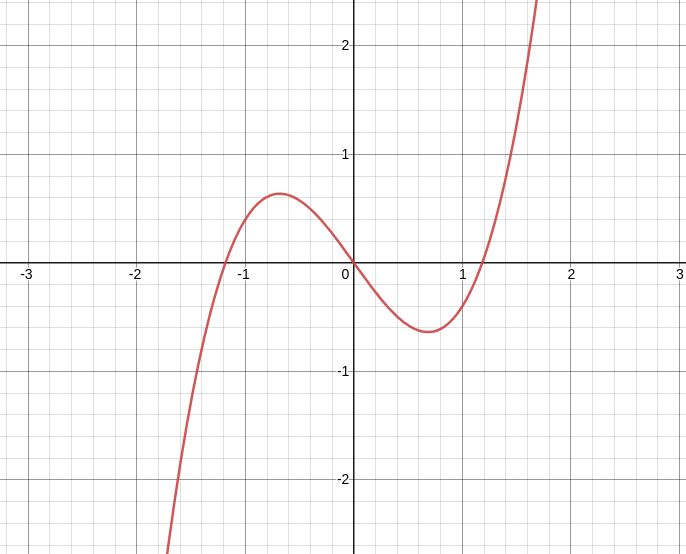
\includegraphics[scale=0.15]{figures/hP.png}
\caption{$x > 0$}
\label{fig:}
\end{subfigure}
\begin{subfigure}[b]{40mm}
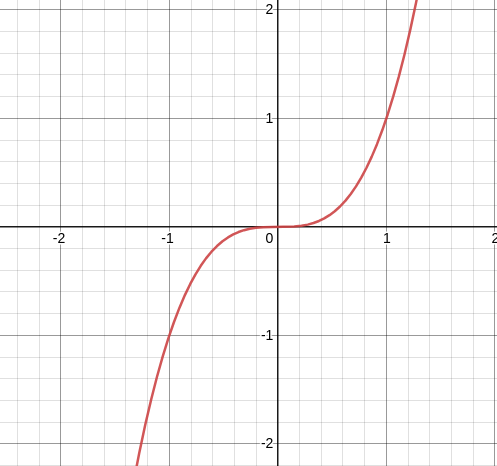
\includegraphics[scale=0.18]{figures/h0.png}
\caption{$x = 0$}
\label{fig:}
\end{subfigure}
\begin{subfigure}[b]{40mm}
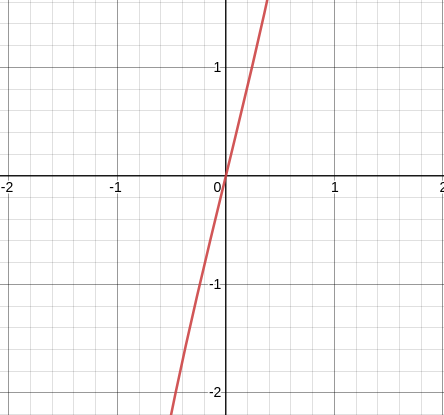
\includegraphics[scale=0.2]{figures/hN.png}
\caption{$x < 0$}
\label{fig:}
\end{subfigure}

\caption{The possible configurations of h}
\label{fig:}
\end{figure}
We find the stationary points of $h(z)$ to be $\pm\sqrt{\frac{x}{3}}$. We find $h^{\prime\prime}(z) = 6z -1$. Note figure 3 where if $x$ is negative we have no stationary points and if $x=0$ we have an inflection point. Then 
\begin{align*}
u(x,t)\rightarrow \left[\frac{2\pi}{|6(\pm \sqrt{\frac{x}{3}} - 1)| \tau} \right]^{\frac{1}{2}} \left[ \frac{A}{2\pi} \frac{\sin\left( \frac{\tau \left(\pm \sqrt{\frac{x}{3}}\right)}{2} \right)}{\left(\pm\sqrt{\frac{x}{3}}\right)} \right ] \exp\left\{i\tau\left(\left(\pm\sqrt{\frac{x}{3}}\right)^3 - \pm\sqrt{\frac{x}{3}}x \right)+ i\frac{\pi}{4}sign\left(6\left(\pm\sqrt{\frac{x}{3}}\right)-1\right)\right\}
\end{align*}
The results in section 4 were obtained by simply plugging in the correct $x$ and $t$ values, note that we move from $tau$ back to $t$.
\section{Results}
Code for the generation of asymptotic behavior figures can be found \href{https://github.com/Liam-Watson/Analysis-of-mKdV-equation-with-Heaviside-IC/blob/main/asym.m}{here} and the influence function \href{https://github.com/Liam-Watson/Analysis-of-mKdV-equation-with-Heaviside-IC/blob/main/integral.m}{here}.
\begin{figure}[H]
\centering
\begin{subfigure}[b]{85mm}
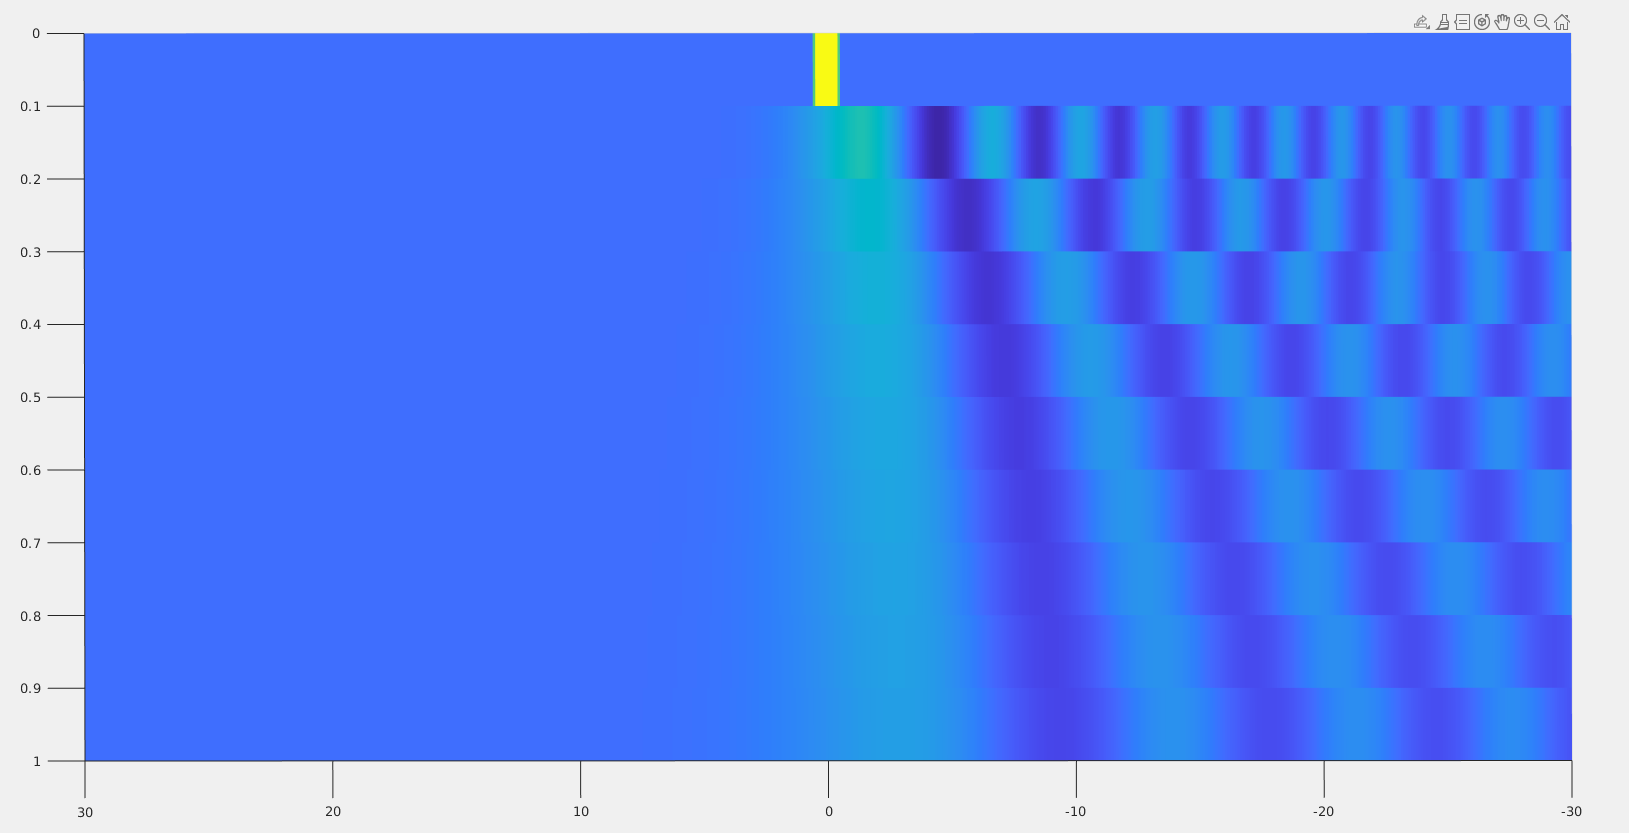
\includegraphics[scale=0.14]{figures/infl0p5H.png}
\caption{A = 0.5}
\label{fig:}
\end{subfigure}
\begin{subfigure}[b]{85mm}
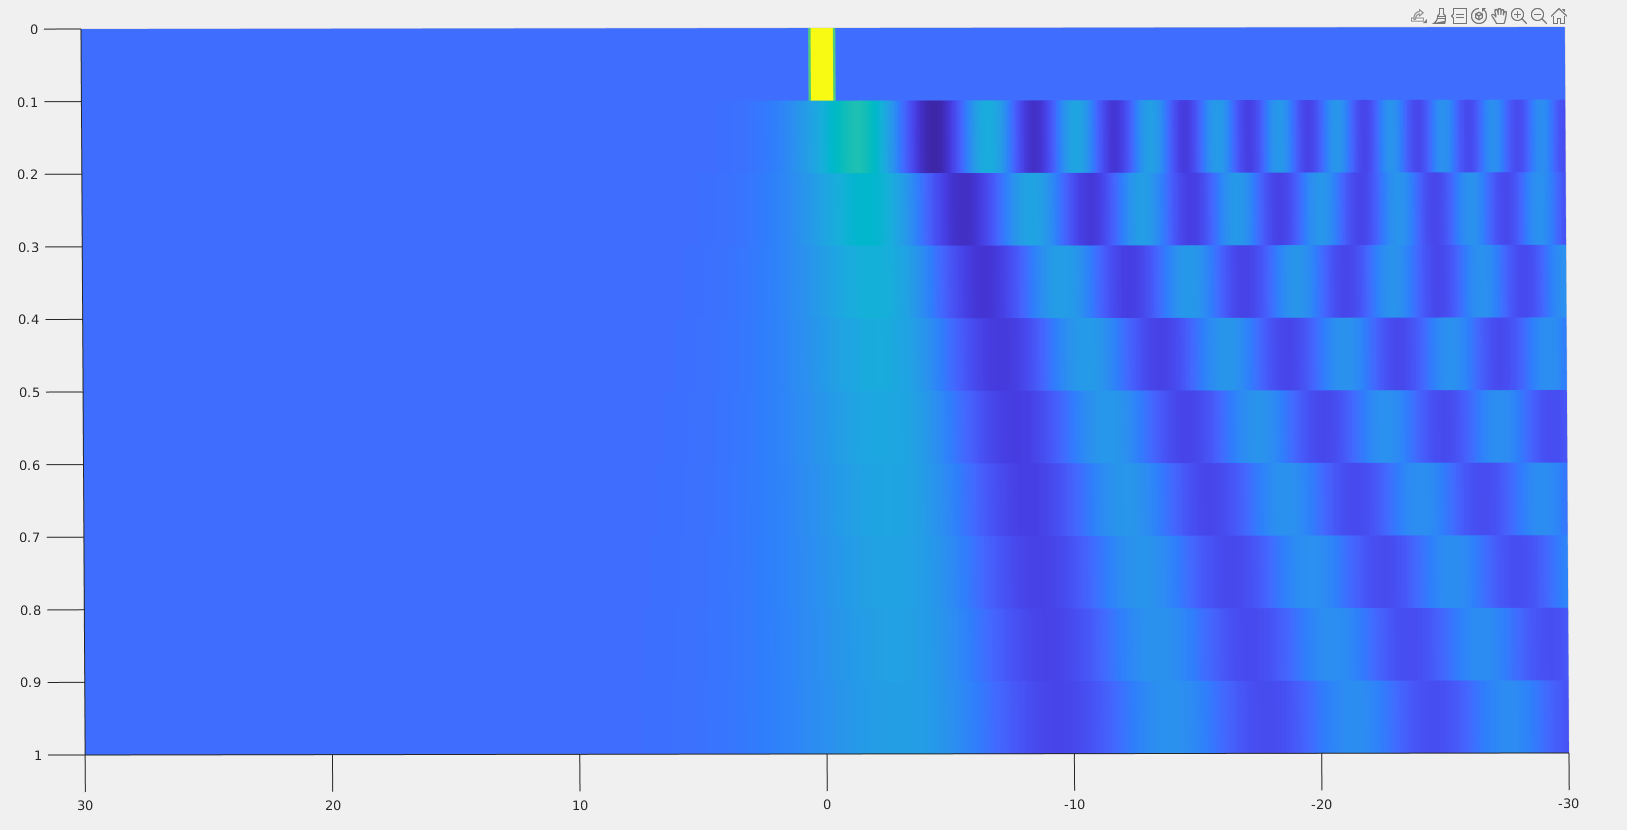
\includegraphics[scale=0.14]{figures/infl1H.png}
\caption{A = 1}
\label{fig:}
\end{subfigure}
\begin{subfigure}[b]{85mm}
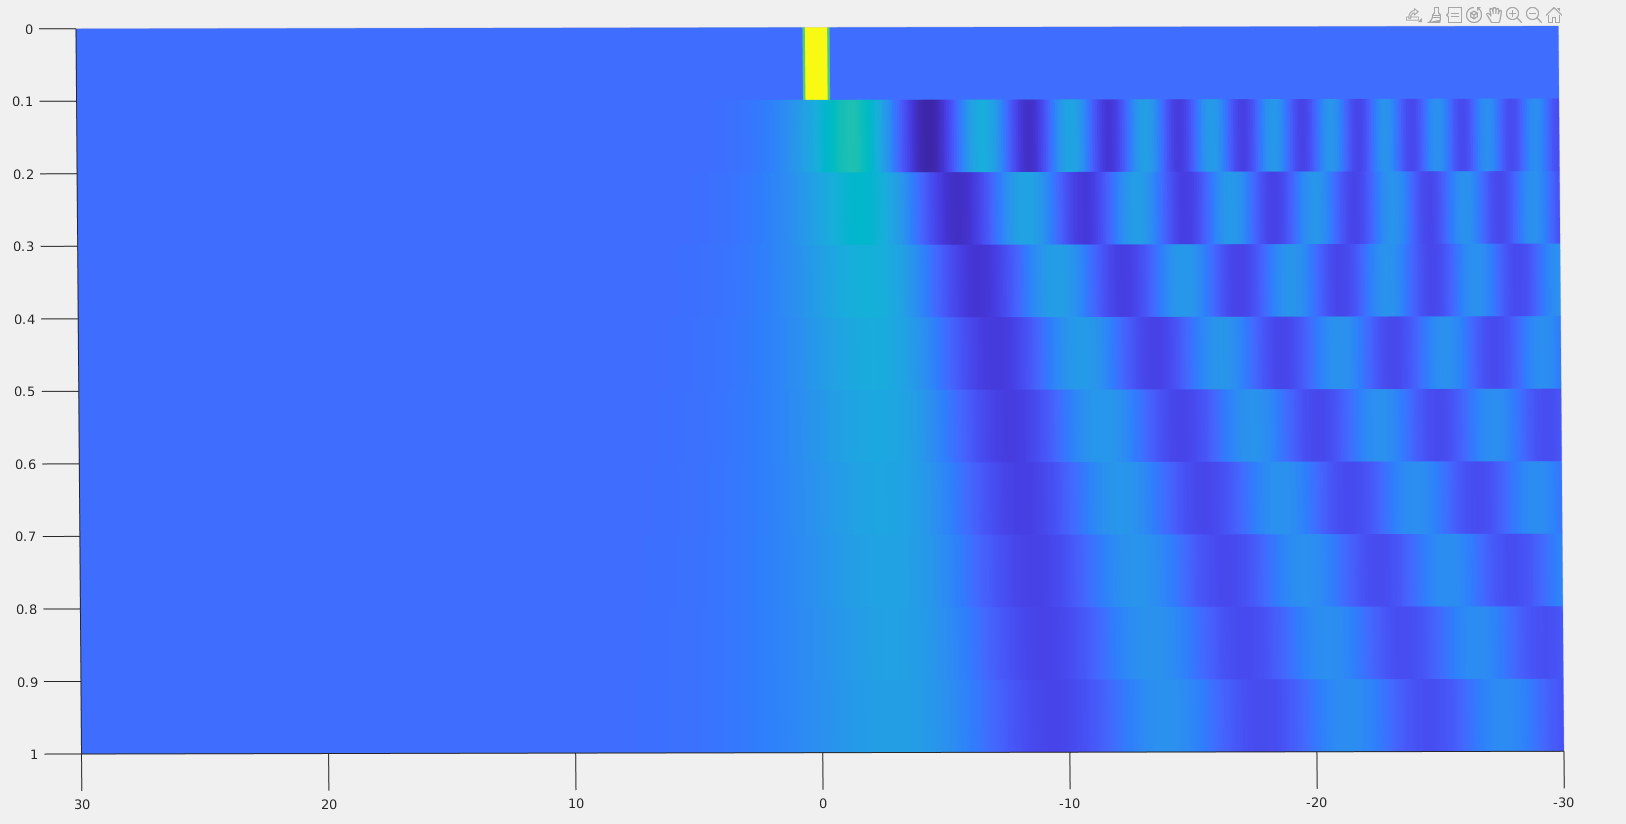
\includegraphics[scale=0.14]{figures/infl1p5H.png}
\caption{A = 1.5}
\label{fig:}
\end{subfigure}
\begin{subfigure}[b]{85mm}
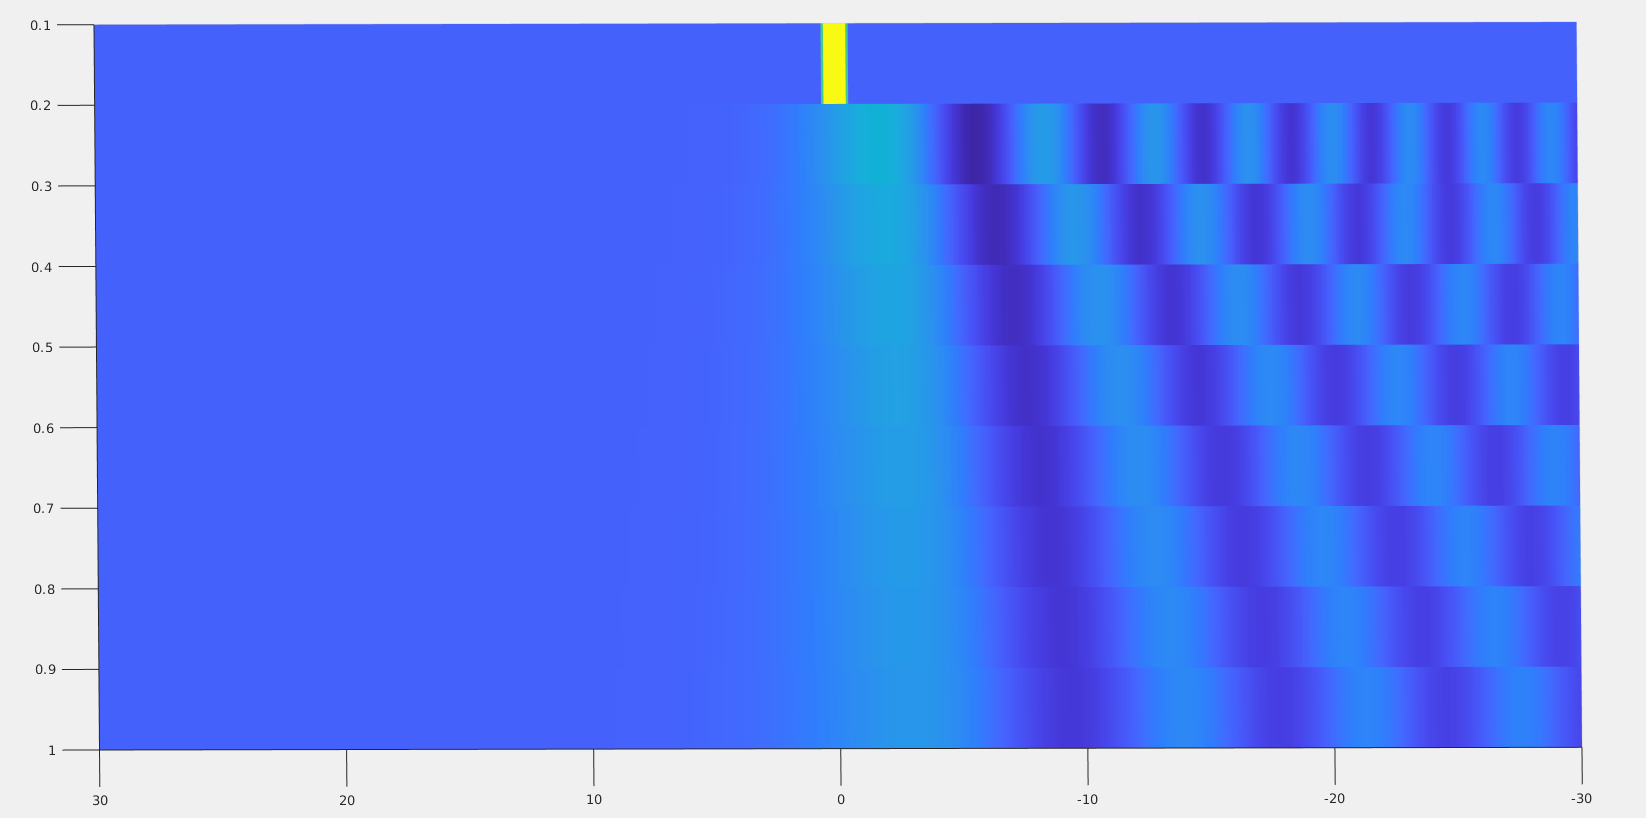
\includegraphics[scale=0.14]{figures/infl2H.png}
\caption{A = 2}
\label{fig:}
\end{subfigure}

\caption{Heat map of the influence function solution showing that as A grows the oscillations are increasingly dispersed or "smoothed", this is evident from the wider waves in sub figure (d) than the other sub figures}
\label{fig:}
\end{figure}

\begin{figure}[H]
\centering
\begin{subfigure}[b]{85mm}
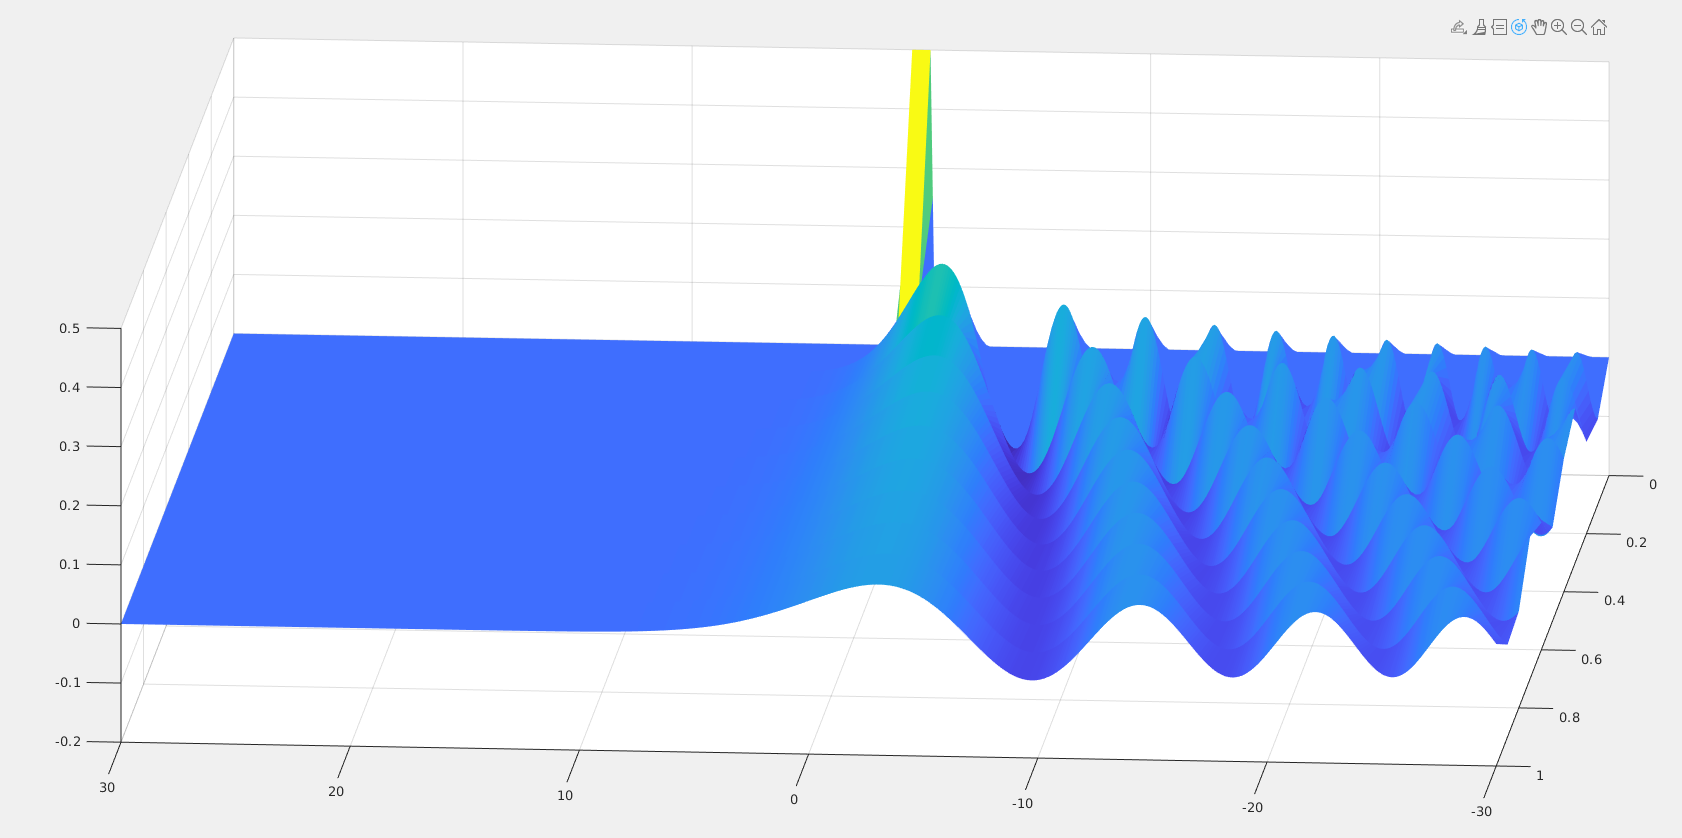
\includegraphics[scale=0.14]{figures/infl0p5V.png}
\caption{A = 0.5}
\label{fig:}
\end{subfigure}
\begin{subfigure}[b]{85mm}
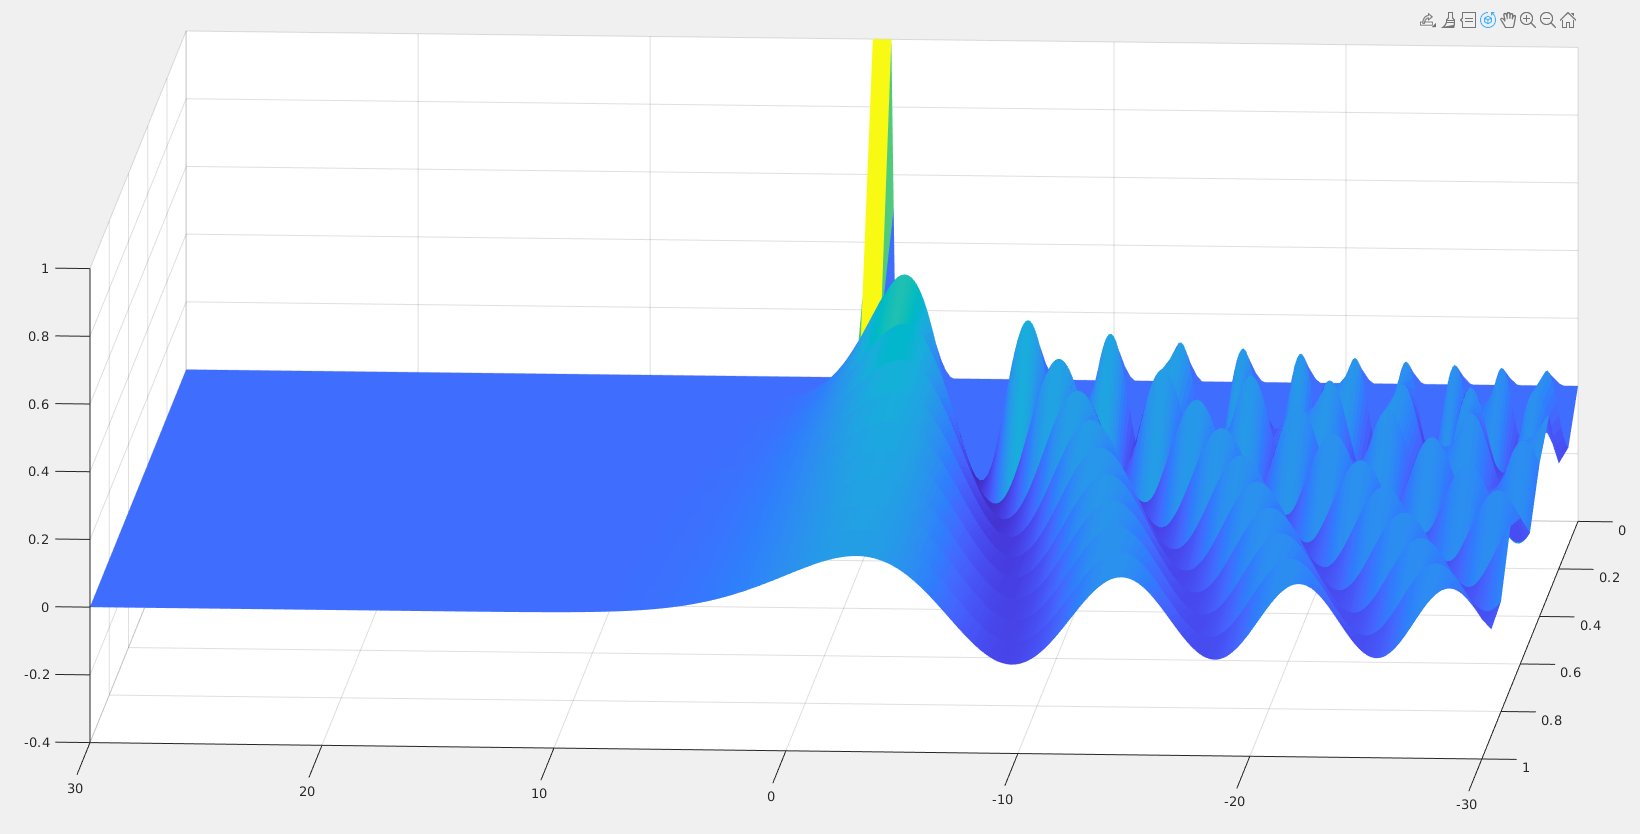
\includegraphics[scale=0.14]{figures/infl1V.png}
\caption{A = 1}
\label{fig:}
\end{subfigure}
\begin{subfigure}[b]{85mm}
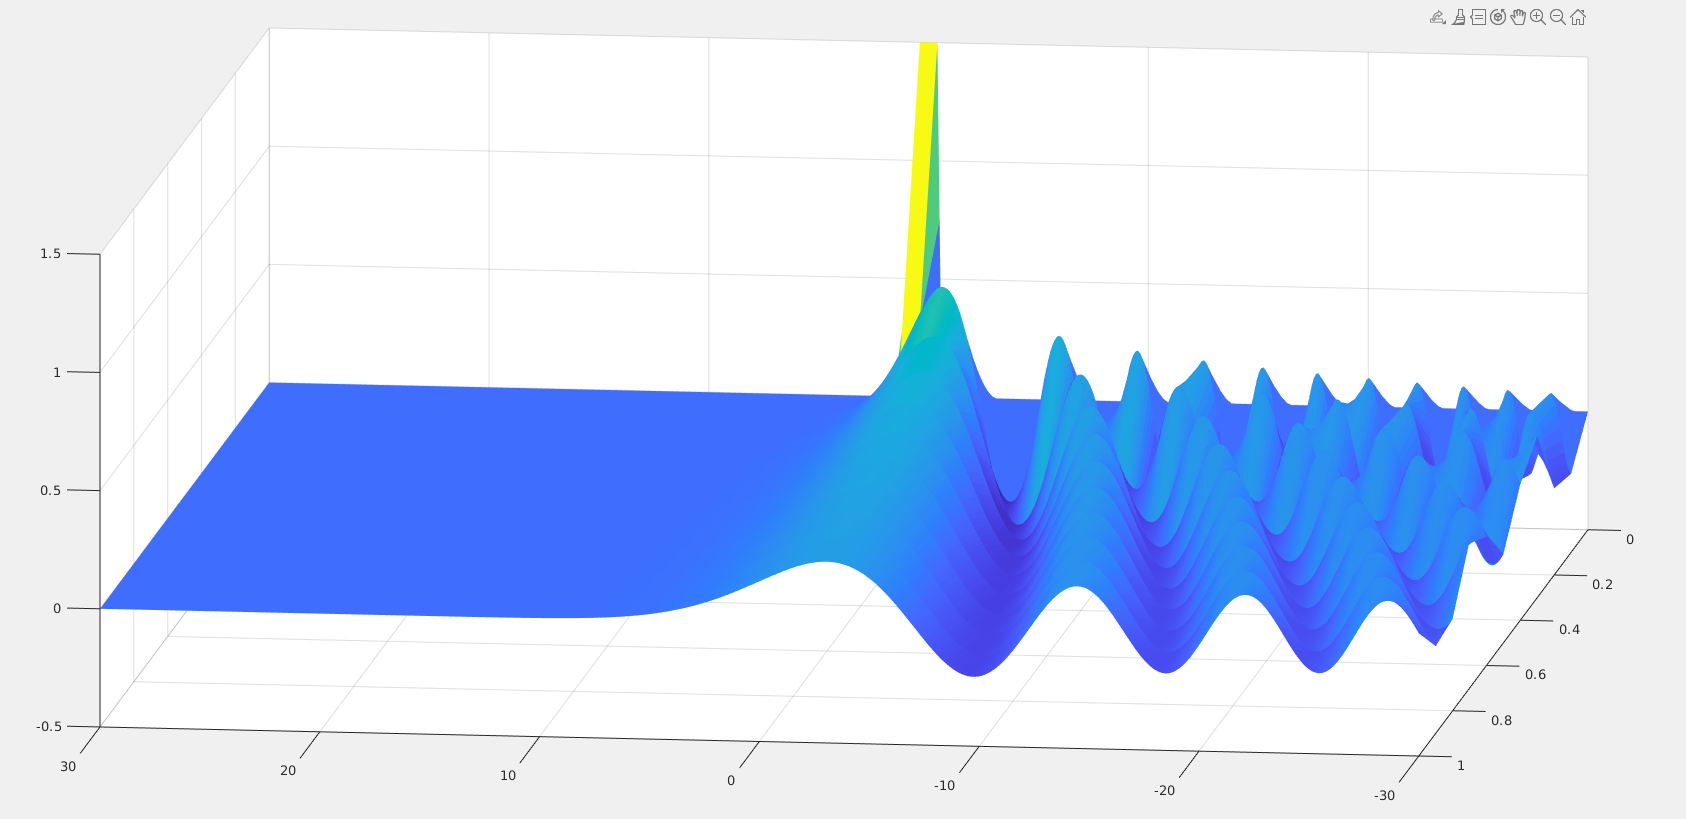
\includegraphics[scale=0.14]{figures/infl1p5V.png}
\caption{A = 1.5}
\label{fig:}
\end{subfigure}
\begin{subfigure}[b]{85mm}
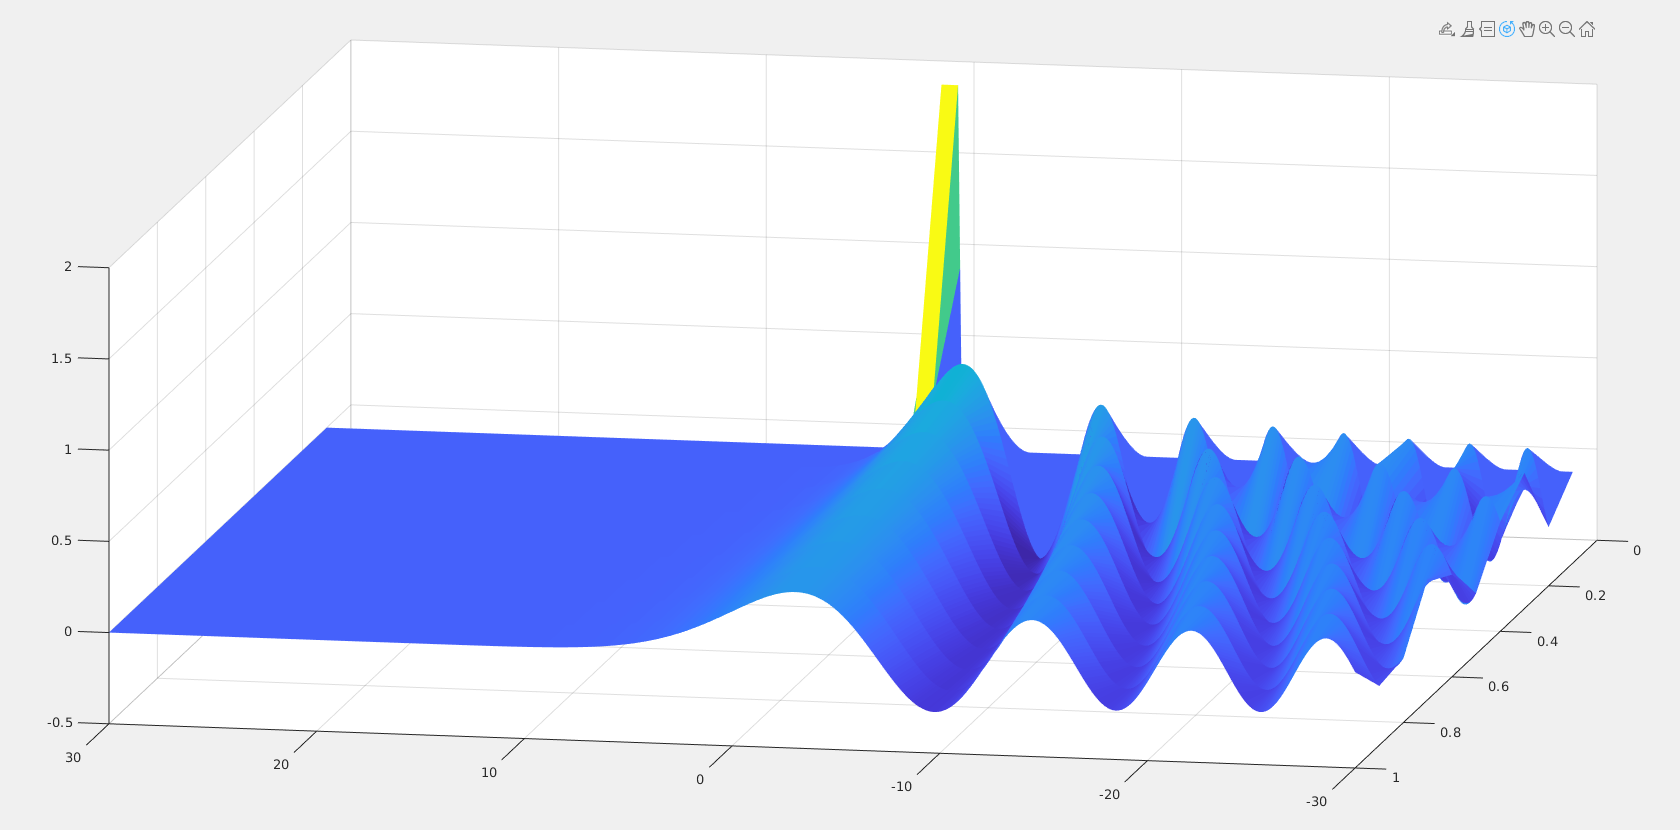
\includegraphics[scale=0.14]{figures/infl2V.png}
\caption{A = 2}
\label{fig:}
\end{subfigure}

\caption{Surface plot of the influence function solution which shows that the behavior of the solution is similar across the tested ranges of A}
\label{fig:}
\end{figure}

\begin{figure}[H]
\centering
\begin{subfigure}[b]{85mm}
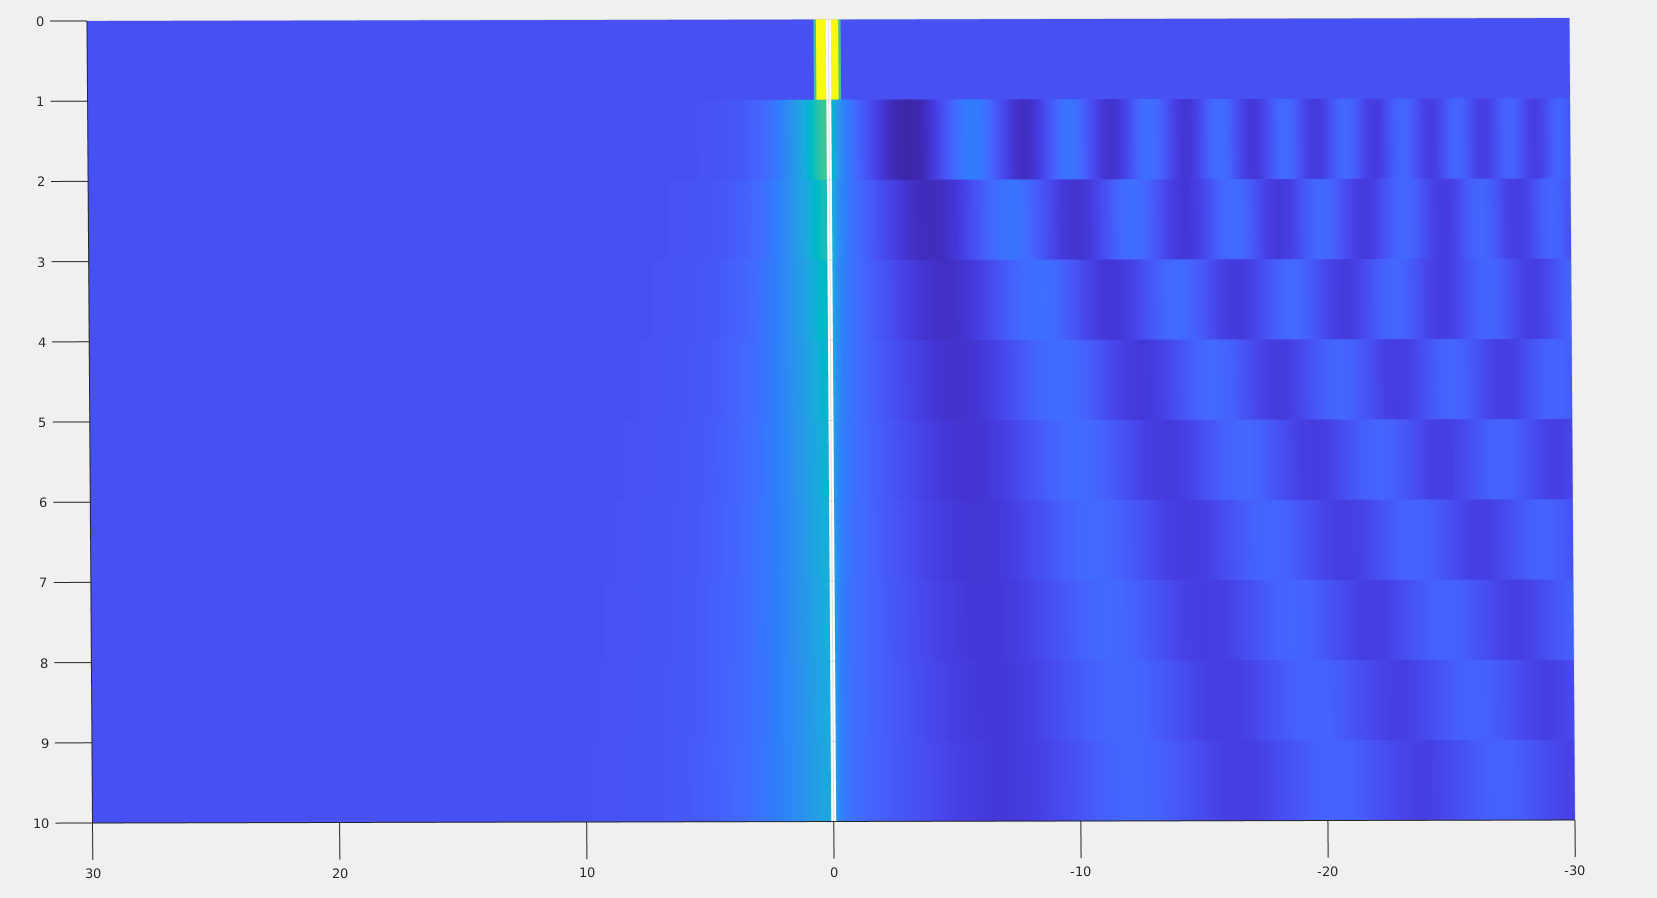
\includegraphics[scale=0.14]{figures/asym0p5H.png}
\caption{A = 0.5}
\label{fig:}
\end{subfigure}
\begin{subfigure}[b]{85mm}
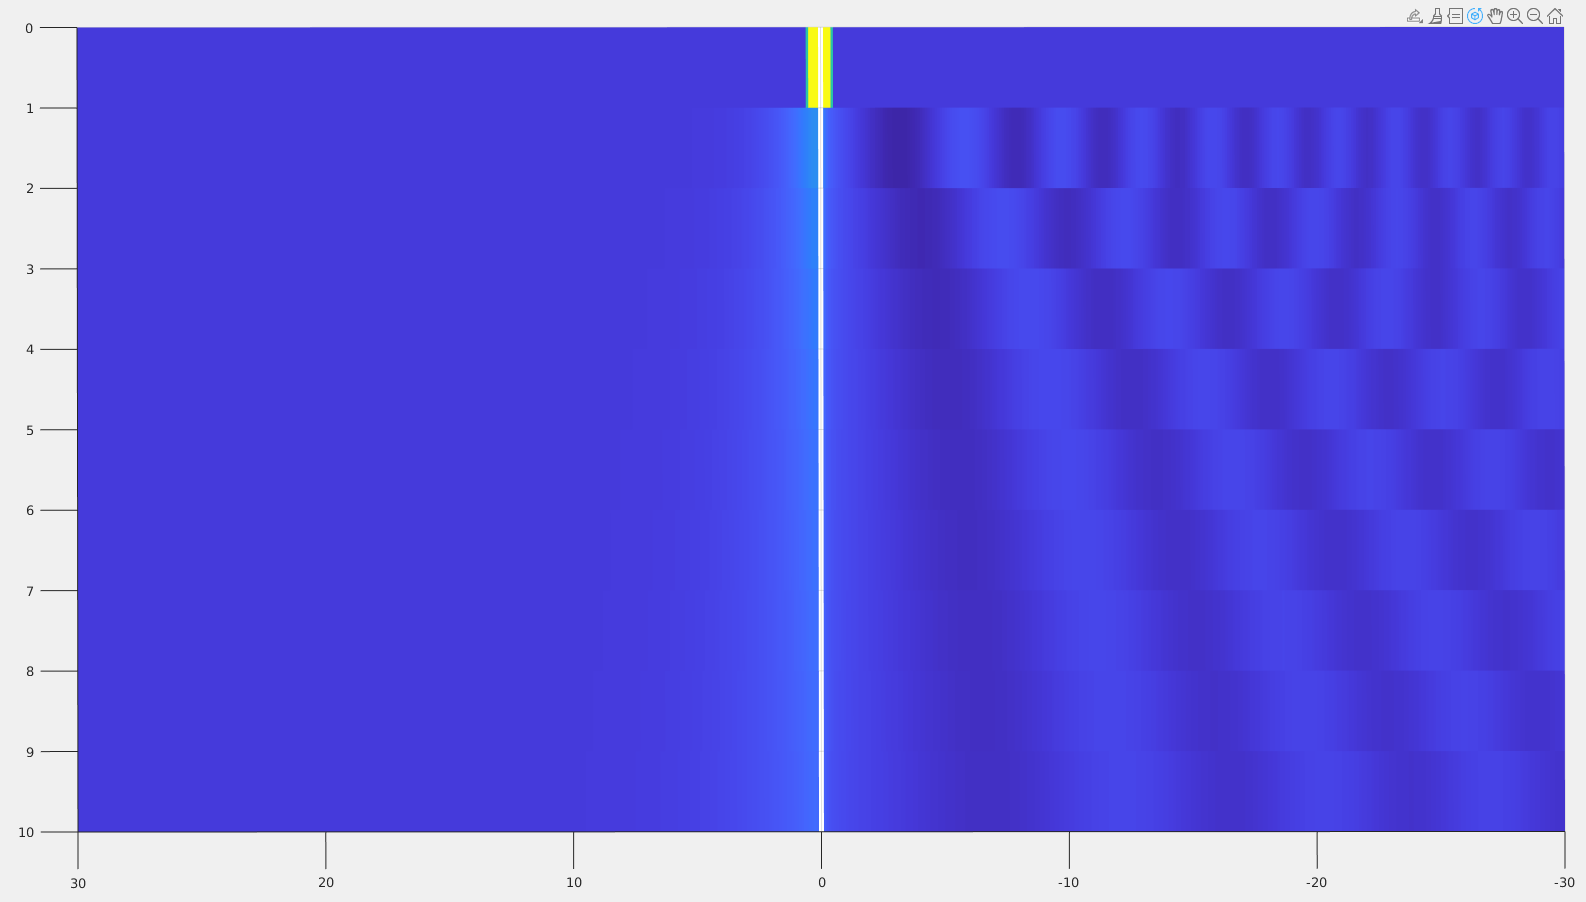
\includegraphics[scale=0.14]{figures/asym1H.png}
\caption{A = 1}
\label{fig:}
\end{subfigure}
\begin{subfigure}[b]{85mm}
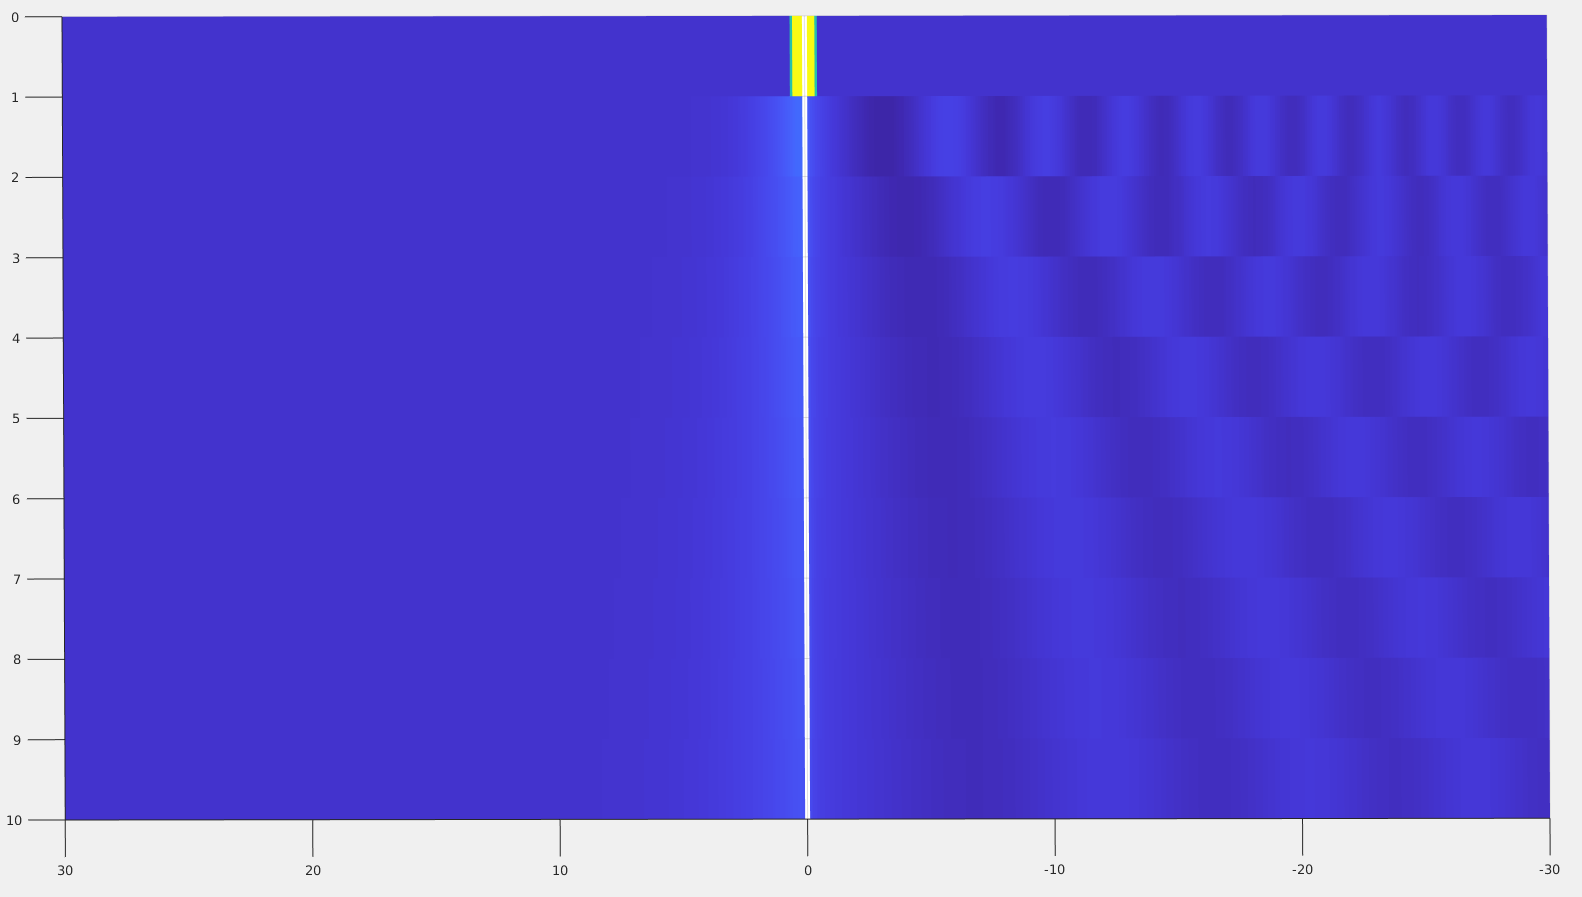
\includegraphics[scale=0.14]{figures/asym1p5H.png}
\caption{A = 1.5}
\label{fig:}
\end{subfigure}
\begin{subfigure}[b]{85mm}
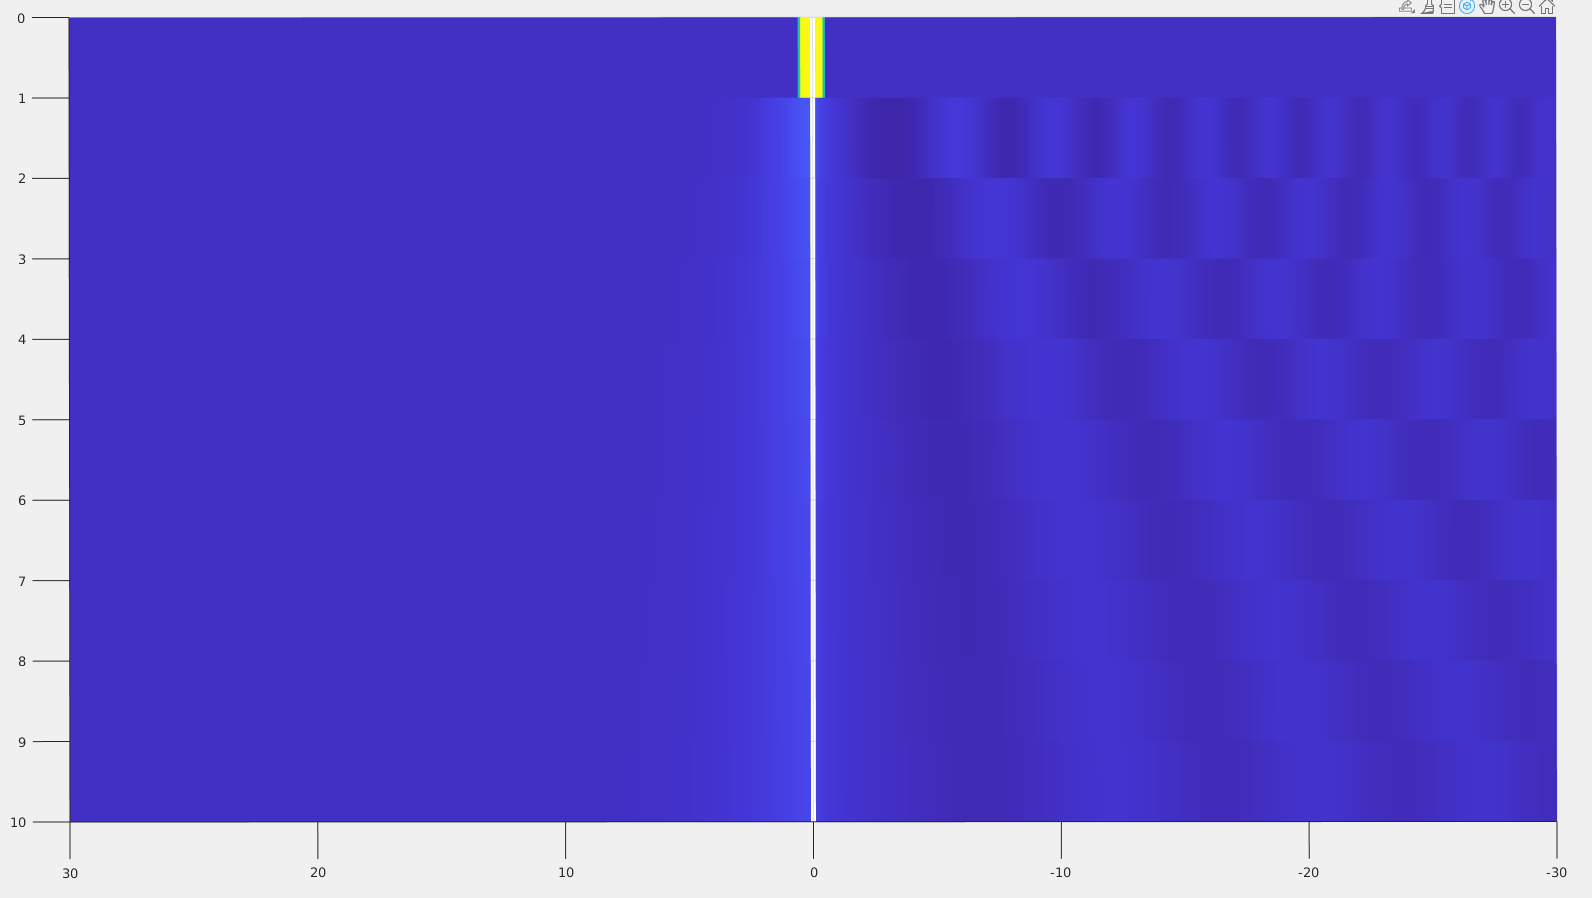
\includegraphics[scale=0.14]{figures/asym2H.png}
\caption{A = 2}
\label{fig:}
\end{subfigure}


\caption{Heat map plot of the the asymptotic expansion solution to the linearized KdV equation. Note the white bar at $x=0$, this is because the asymptotic expansion is not defined. There is no need to show the surface plot as the behavior can be inferred from the other surface plot and heat map pairs in figures 4/5 and 2}
\label{fig:}
\end{figure}

\section{Numerical and analytical comparison}
\subsection{Comparing the asymptotic expansion to influence function solution}
From figures 4 and 6 we can see that both solutions show the same behavior for small and large time scales with the square pulse dispersing into progressively smaller waves in the negative $x$ interval and showing little interesting behavior in the positive $x$ interval. \\
With both solutions as we increase the initial condition amplitude ($A$) we can see the rate of dispersion increase with the amplitude of the secondary waves decreasing faster in time than with small values of $A$. It is interesting to note that these solutions are so similar given that the asymptotic expansion is an approximation where as the influence function solution was solved using symbolic integration and hence is nearly exact. The main difference of note is that the asymptotic solution disperses more quickly than the influence function solution which is evident in the heat maps of figures 6 and 4, this is likely due to the asymptotic expansion displaying the behavior of the solution for large time values. \\
An interesting feature of the influence function is that is "blows up" for very small time values whereas the asymptotic expansion does not.
\begin{figure}[H]
\centering
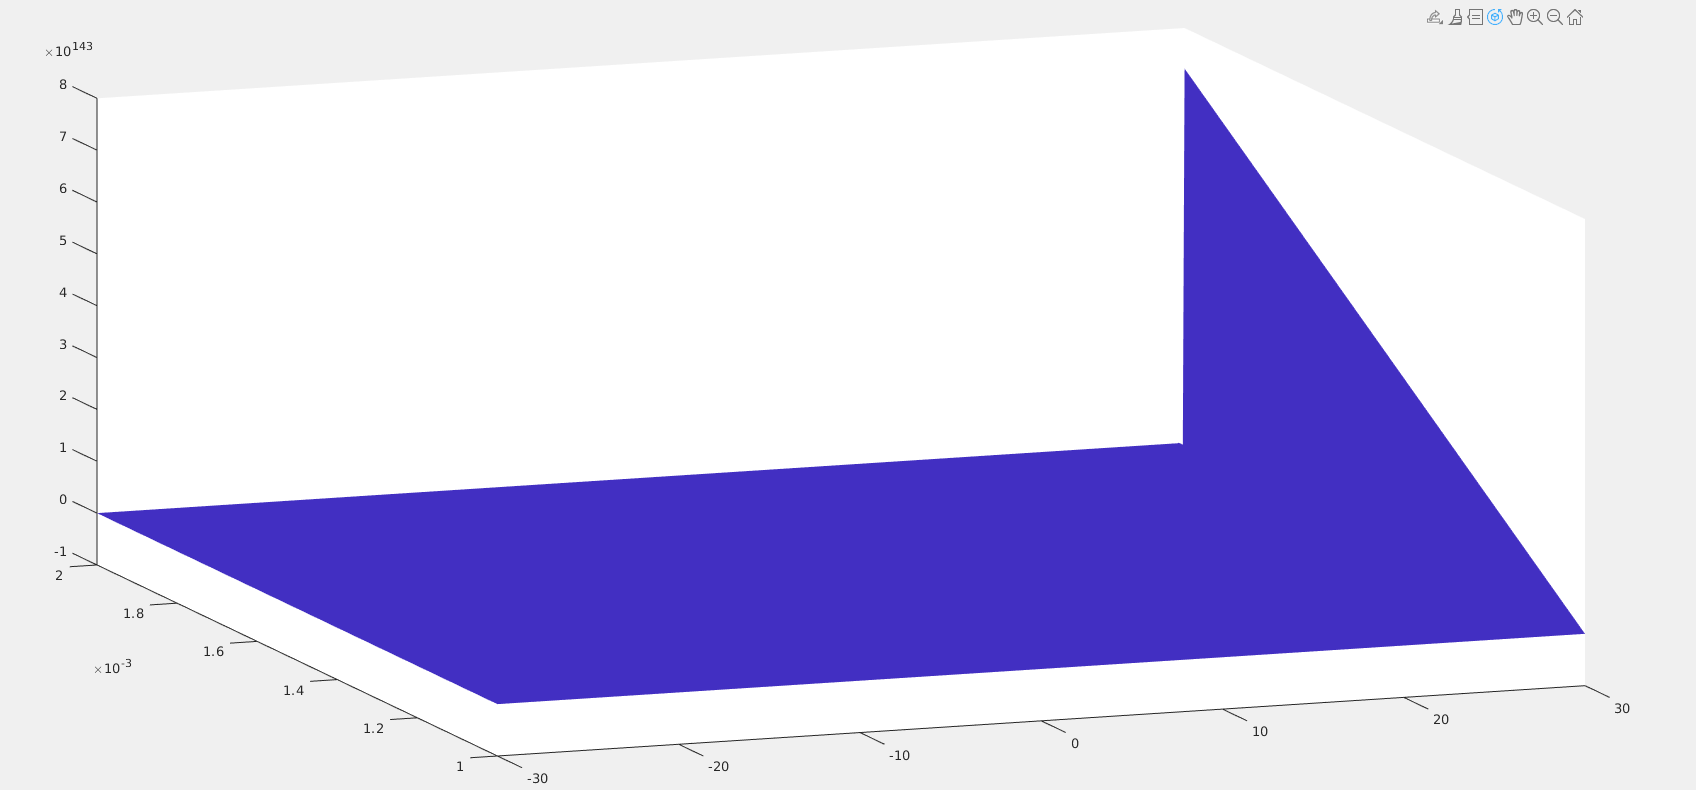
\includegraphics[scale=0.2]{figures/inflSmallT.png}
\caption{Showing that the influence function blows up for small values of time $t \sim 10^-3$}
\label{fig:}
\end{figure}

\subsection{Numerical solution versus analytical solutions}
Figure 2(b), displays the behavior of the numerical solution in time as a surface, from which we can tell that the initial square pulse disperses into many smaller waves in the negative $x$ interval (after we undo the x-shift that was applied for numeric reasons) with these dispersive waves decreasing in amplitude in both the negative $x$ and time directions which is precisely the behavior we see from the analytical solutions. However, the dispersive waves are of a much lower frequency in the numerical solution when we account for the scale of the x-axis, this is likely due to the increased interval and is not representative of the actual qualitative behavior of the solution. An additional insight from the surface and heat map plots is that the frequency of the dispersive waves decreases in time. This is especially evident for small time values where we can see the waves are densely packed and as $t$ grows the waves spread out.\\
The numerical solution does perform better in cases where the two analytical solutions fail: the asymptotic solutions are undefined at $x=0$ and if we look back to figure 7 we can see that the influence function does not deal well with small time values ($\sim 10^{-3}$) but the numerical and asymptotic solutions do.
\section{final remarks and conclusions}
It is surprising to see how well the asymptotic expansion matched the qualitative behavior of the numerical and influence function solutions. With that said it is unfortunate that the approximation produced by the method of stationary phase is undefined at $x=0$, it is possible a different method of asymptotic expansion would mend this issue. \\
Additionally it was insightful to see that although the Heaviside initial condition seems dangerously resistant to numerical integration we were able to integrate it by using a fine $x$ and time mesh, shifting the origin to the positive $x$ interval and increasing the simulation interval $L$. \\
The solution plots we have obtained are all very similar, good, but what do they physically mean. The mKdV equation is used to model plasma's and solid-state physics phenomena and we can interpret our solution as starting with a single high energy region that "ripples" throughout the plasma or solid in dispersive waves until an energy equilibrium is reached, rather than uniformly decaying like a solution to the heat equation might. Physically I struggle to interpret the behavior of the positive x region, however, this possibly requires further investigation which is beyond the scope of this paper. 

\section{Acknowledgements}
A sincere thanks to:\\
Dean Reagon for willing to bounce solutions off each other.\\
Emma Gamble for her homework assignment 2.6 answer on the QnA. \\
Louis De Jager for his homework assignment 1.3 answer on the QnA.  \\
\end{document}